
%===========================================================================
\section{Analisis Kesalahan} \label{IV.AnalisisKesalahan}
%===========================================================================

Bagian ini menyajikan analisis mendalam terhadap pola kesalahan klasifikasi yang masih terjadi meskipun model telah mencapai performa optimalnya. Analisis ini bertujuan untuk memahami karakteristik spesifik dari sampel-sampel yang gagal diprediksi dengan benar, sehingga dapat memberikan wawasan mengenai batasan kemampuan arsitektur model serta kompleksitas visual dan temporal dari kelas-kelas tertentu dalam dataset SIBI. Melalui telaah \textit{confusion matrix} dan observasi kualitatif terhadap frame video, evaluasi difokuskan untuk mengidentifikasi kelas-kelas yang secara persisten menjadi sumber \textit{misclassification} utama.\par

Meskipun seluruh model mencapai akurasi tinggi, dua kelas yang secara konsisten menunjukkan F1-\textit{score} terendah di semua arsitektur adalah Suka dan Mau. Pada E12, Suka memperoleh F1 0{,}91 dan Mau memperoleh F1 0{,}90, keduanya paling rendah dibandingkan kelas lain meskipun masih tergolong tinggi secara absolut. Pola ini konsisten dengan temuan pada model sebelumnya: Suka pada E9 mencapai F1 0{,}53 sementara mayoritas kelas sudah di atas 0{,}60, dan pada E5 nilai Mau (F1 0{,}52) dan Suka (F1 0{,}31) tertinggal jauh dari kelas lain. Analisis \textit{confusion matrix} memperlihatkan bahwa sebagian sampel Suka cenderung terprediksi sebagai Mau, dan sebaliknya, sehingga pasangan ini merupakan sumber \textit{misclassification} yang paling persisten bahkan setelah performa model secara umum sudah sangat tinggi.\par

Secara visual, kemiripan tersebut dapat dipahami dari contoh frame representatif: baik Mau maupun Suka sama-sama menempatkan tangan dominan pada area artikulasi tengah, yakni sekitar dada hingga perut, dengan tubuh menghadap kamera dan latar yang seragam. Pada level citra tunggal, keduanya tidak memiliki pembeda kasar yang setajam kelas seperti Bawa atau Guru. Hal ini penting karena menunjukkan bahwa satu frame statis saja sering belum cukup untuk membedakan kedua kata tersebut; sinyal pembeda utama justru terletak pada bagaimana tangan bergerak dari posisi awal menuju posisi akhir. Gambar~\ref{fig:4.mau_vs_suka} menunjukkan perbandingan visual sampel gerakan dari kelas Mau dan Suka.\par

\begin{figure}[H]
\centering
\makebox[\textwidth][c]{\begin{minipage}{1.1\textwidth}
\centering
% Row 1: Mau
\begin{subfigure}[b]{0.24\linewidth}
  \centering
  
\includegraphics[width=\linewidth]{figure/sampel_blurred/Mau_099_sample1.png}
  \caption{Mau (Sampel 1)}
\end{subfigure}
\hfill
\begin{subfigure}[b]{0.24\linewidth}
  \centering
  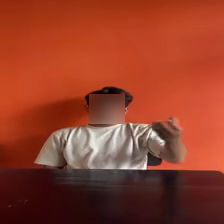
\includegraphics[width=\linewidth]{figure/sampel_blurred/Mau_099_sample2.png}
  \caption{Mau (Sampel 2)}
\end{subfigure}
\hfill
\begin{subfigure}[b]{0.24\linewidth}
  \centering
  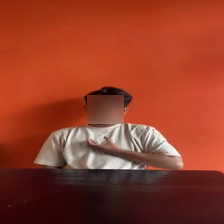
\includegraphics[width=\linewidth]{figure/sampel_blurred/Mau_099_sample3.png}
  \caption{Mau (Sampel 3)}
\end{subfigure}
\hfill
\begin{subfigure}[b]{0.24\linewidth}
  \centering
  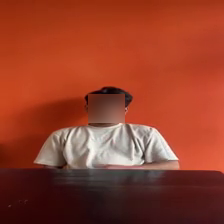
\includegraphics[width=\linewidth]{figure/sampel_blurred/Mau_099_sample4.png}
  \caption{Mau (Sampel 4)}
\end{subfigure}
\vspace{0.5cm}

% Row 2: Suka
\begin{subfigure}[b]{0.24\linewidth}
  \centering
  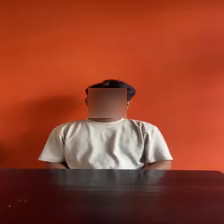
\includegraphics[width=\linewidth]{figure/sampel_blurred/Suka_090_sample1.png}
  \caption{Suka (Sampel 1)}
\end{subfigure}
\hfill
\begin{subfigure}[b]{0.24\linewidth}
  \centering
  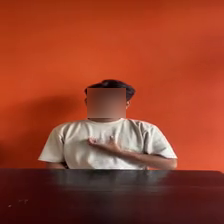
\includegraphics[width=\linewidth]{figure/sampel_blurred/Suka_090_sample2.png}
  \caption{Suka (Sampel 2)}
\end{subfigure}
\hfill
\begin{subfigure}[b]{0.24\linewidth}
  \centering
  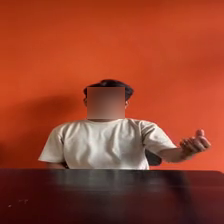
\includegraphics[width=\linewidth]{figure/sampel_blurred/Suka_090_sample3.png}
  \caption{Suka (Sampel 3)}
\end{subfigure}
\hfill
\begin{subfigure}[b]{0.24\linewidth}
  \centering
  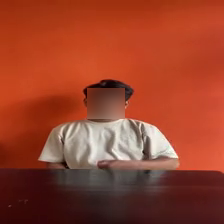
\includegraphics[width=\linewidth]{figure/sampel_blurred/Suka_090_sample4.png}
  \caption{Suka (Sampel 4)}
\end{subfigure}
\end{minipage}}
\captionsetup{justification=raggedright,singlelinecheck=false}
\caption{Perbandingan visual sampel gerakan gestur Mau (baris atas) dan Suka (baris bawah)}
\label{fig:4.mau_vs_suka}
\end{figure}

Kondisi ini menegaskan bahwa untuk bahasa isyarat, model tidak bisa hanya mengandalkan fitur spasial tunggal. Kemampuan model untuk menangkap \textit{temporal dynamics}---perubahan antar-frame---menjadi sangat krusial. Pada kelas Mau dan Suka, model sering kali 'bingung' karena keduanya memiliki fitur spasial yang identik pada frame-frame tertentu, dan hanya dibedakan oleh kecepatan atau arah pergerakan yang sangat halus. Ini adalah tantangan utama dalam \textit{fine-grained action recognition}, di mana kelas-kelas tertentu memerlukan \textit{temporal receptive field} yang lebih panjang atau mekanisme \textit{attention} yang lebih sensitif terhadap perubahan kecil di sepanjang waktu. Kesalahan yang terjadi pada kelas ini sebagian besar adalah masalah dinamika gestur daripada masalah bentuk pose tunggal.\par

Secara temporal, kedua gestur sama-sama memuat lintasan tangan pendek di ruang artikulasi yang berdekatan, sehingga perbedaannya bertumpu pada detail mikro seperti arah lintasan akhir, besar amplitudo gerak, perubahan orientasi telapak, dan \textit{timing} saat tangan berhenti. Jika model gagal menangkap salah satu fase tersebut, maka representasi kedua kelas menjadi sangat berdekatan di ruang fitur. Gejala ini terlihat jelas pada E10, di mana \textit{dense sampling} menurunkan F1 kelas Suka hingga 0{,}14 dan banyak sampelnya diprediksi sebagai Mau atau Kamu; hal ini mengindikasikan bahwa ketika cakupan temporal tidak lengkap, petunjuk pembeda pada fase awal atau akhir gestur mudah hilang. Sebaliknya, pada E12, ViViT, dan I3D, kesalahan tinggal tersisa dalam jumlah kecil, tetapi tetap terkonsentrasi pada dua kelas ini, yang menunjukkan bahwa bahkan model dengan representasi spasio-temporal kuat masih harus bekerja lebih keras untuk membedakan pola gerak yang sangat mirip secara lokal.\par

Dari sudut pandang linguistik bahasa isyarat, temuan ini memperlihatkan bahwa Mau dan Suka berbagi parameter manual tingkat tinggi yang serupa, tetapi dibedakan oleh konfigurasi sub-gerak yang lebih halus. Karena itu, kesalahan klasifikasi keduanya bukan sekadar akibat kekurangan data, melainkan mencerminkan batas diskriminasi model terhadap isyarat yang memiliki kemiripan lokasi artikulasi dan orientasi awal. Analisis ini memberi bobot ilmiah tambahan pada hasil penelitian: untuk tugas pengenalan SIBI berbasis video, evaluasi tidak cukup berhenti pada akurasi global, tetapi perlu menelaah pasangan kelas yang secara linguistik dan visual berdekatan. Perbaikan lebih lanjut pada pasangan Mau--Suka kemungkinan memerlukan penambahan sampel dengan variasi lintasan gerak yang lebih kaya, resolusi temporal yang lebih padat namun tetap mencakup keseluruhan gestur, atau pendekatan yang lebih eksplisit memodelkan pose tangan dan perubahan orientasi antar-frame.\par

